\chapter{使用\LaTeX{}进行文档编辑}
\label{cp:latex}

\section{基本常识}

\LaTeX{}是一种基于\TeX{}的排版系统,提供了一种\textbf{类似于标签语言}的文档编辑方式,我们通过\textbf{源代码}来控制文档的排版效果,此外,通过\textbf{命令}则可以控制文档的格式、结构、样式等,预定义好了这些设定(或使用编写好的模板),我们便不需要关心具体的排版细节。\LaTeX{}的结构严谨性及对公式表达的良好支持,使它科学、学术和出版等领域应用广泛。\\

正如\nameref{cp:abstract}中所述,在对\LaTeX{}的实践中,我深入了对该语言的认知。在编辑器选择上,我偏向于使用本地编译\footnote{Overleaf提供的在线编辑器常出现编译时间过长问题,可能是由于我的模板较为复杂,另外免费版无法托管至GitHub,故而弃用。在本地编写编译更方便,还可以托管到GitHub库中进行版本控制。},采用\textit{TeX Live}引擎,利用\textit{VS Code}进行。\\

本章所有对\LaTeX{}的解释,都出自于我逐步积累的经验(例如本文章的写作就积累了不少经验)。我将基本概括\LaTeX{}的基本知识,包括\textit{基本结构}、\textit{命令和宏包(Packages)}、\textit{样式设定}、\textit{插图表格}、\textit{参考文献}等。\\

对本模板的维护历史,请您前往我的\href{https://github.com/jstar0/LaTeXTemplate}{GitHub仓库}查看。下面提供Commit记录截图:

\begin{figure}[h!]
    \centering
    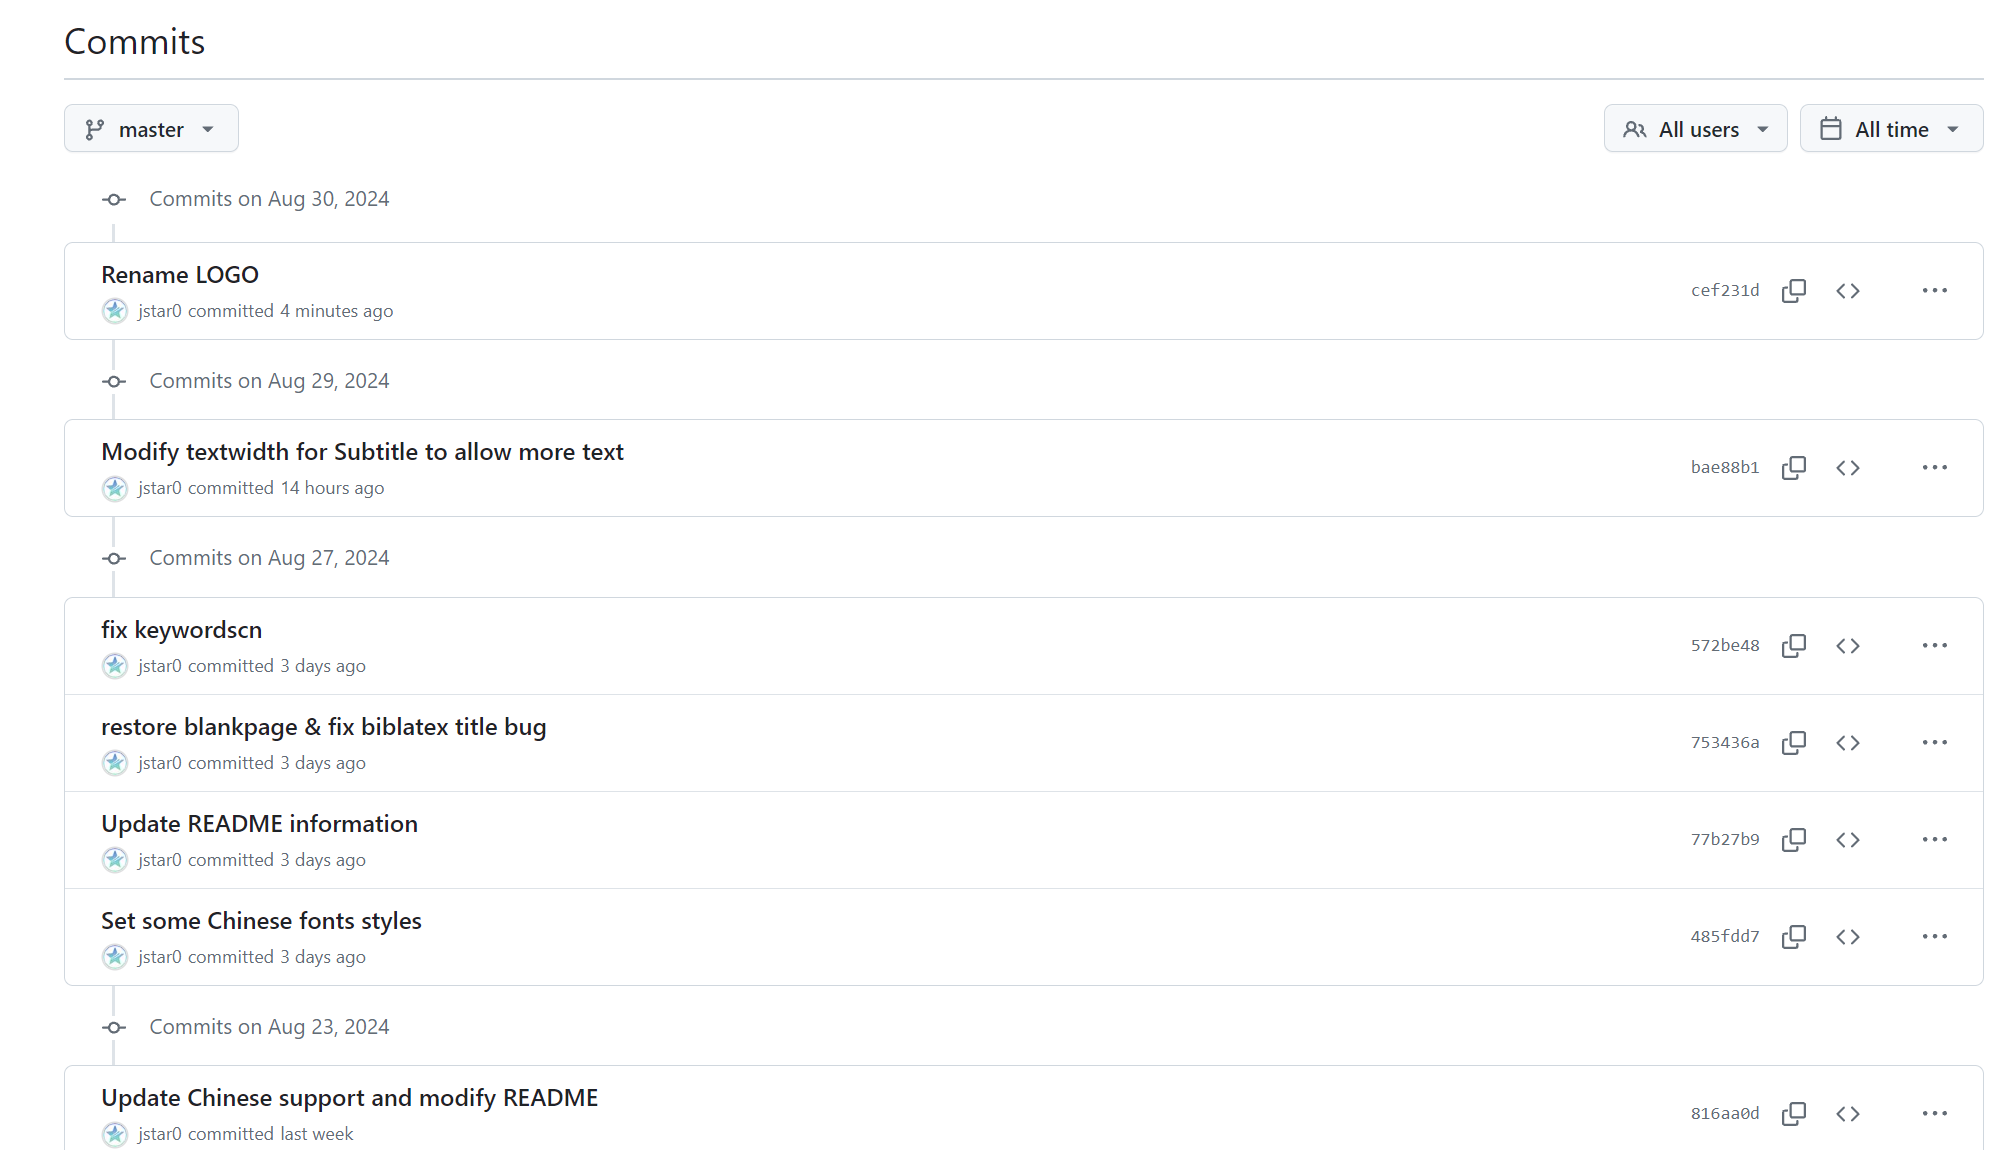
\includegraphics[width=0.8\textwidth]{Figures/git-latex-history.png}
    \caption{模板维护历史}
    \label{fig:git-history}
\end{figure}

\section{基本结构}

\LaTeX{}的文档结构主要包括\textbf{导言区}和\textbf{正文区},导言区用于设置文档的格式、样式、引入宏包等,正文区用于书写文档内容。导言区一般以\texttt{*.cls}或\texttt{*.sty}文件为主,正文区则以\texttt{*.tex}文件为主。在简单的文档中,我们可以将导言区和正文区写在同一个文件中,但在复杂的文档中,我们可以将导言区和正文区分开,甚至将正文区分为多个文件,通过\verb|\input{}|或\verb|\include{}|命令引入。\footnote{本模板就是将导言区和正文区分开的,导言区在\textit{ThesisTemplate.cls}中,正文区在\textit{MainPage.tex}中。而正文区又引用了其他多个\texttt{*.tex}文件。}这种解耦合的方式,使得文档结构更加清晰,易于维护。\\

对我的模板进行\texttt{tree /f}命令,可以发现:

\begin{longlisting}
    \begin{minted}{shell}
        D:.
        |  .gitignore
        |  MainPage.pdf
        |  MainPage.tex
        |  README.md
        |  ThesisTemplate.cls
        |
        --Assets
        --Bibliography
        |      Bibliography.bib
        |
        --Chapters
        |  |  00-Abstract.tex
        |  |  01-Git.tex
        |  |  02-LaTeX.tex
        |  |
        |  --Annexes
        --Figures
        |  |  git-branch-1.png
        |  |  git-local-operations.png
        |  |  github-create-repo.png
        |  |
        |  --Theme
        |          Back-Page-BG.pdf
        |          Cover-BG.pdf
        |          Front-Page-BG.pdf
        |          OUC-Logo-B.pdf
        |          OUC-Logo-W.pdf
        |
        --Matter
        |      00-Cover.tex
        |      01-FPage.tex
        |      02-Declaration.tex
        |      03-Acknowledgements.tex
        |      04-Glossary.tex
        |      05-Acronyms.tex
        |      08-BPage.tex
        |
        --Variables
        |      Variables.tex
        |
        --minted-MainPage
               ....pygtex (省略)
    \end{minted}
    \caption{模板文件结构}
    \label{listing:template-structure}
\end{longlisting}

\section{设置文档、调节字体、字号等}

我们可以通过\verb|\documentclass{}|命令设置文档的类型,例如\textit{article}、\textit{report}、\textit{book}等。对于字体的设定,我们一般使用\textit{xeCJK}宏包,因为他提供了很好的中文支持,并通过\verb|\setmainfont{}|、\verb|\setCJKmainfont{}|等命令设置文档的字体,具体而言:

\begin{longlisting}
    \begin{minted}{latex}
        \documentclass[UTF8]{ctexart}
        \usepackage{xeCJK}
        \setmainfont{Times New Roman}
        \setCJKmainfont{SimSun}
        \setCJKsansfont{SimHei}
        \setCJKmonofont{FangSong}
        \setCJKfamilyfont{zhsong}{SimSun}
        \setCJKfamilyfont{zhhei}{SimHei}
        \setCJKfamilyfont{zhfs}{FangSong}
        \setCJKfamilyfont{zhkai}{KaiTi}
        \setCJKfamilyfont{zhli}{LiSu}
        \setCJKfamilyfont{zhyou}{YouYuan}
        \newcommand*{\songti}{\CJKfamily{zhsong}}
        \newcommand*{\heiti}{\CJKfamily{zhhei}}
        \newcommand*{\kaishu}{\CJKfamily{zhkai}}
        \newcommand*{\fangsong}{\CJKfamily{zhfs}}
        \newcommand*{\lishu}{\CJKfamily{zhli}}
        \newcommand*{\youyuan}{\CJKfamily{zhyou}}
    \end{minted}
    \caption{设置文档字体}
    \label{listing:font-setting}
\end{longlisting}

\section{文本格式控制}

一些基本的命令:\verb|\textit{}|、\verb|\textbf{}|、\verb|\underline{}|等命令可以设置文本的格式,而在中文支持中,斜体一般使用楷体,加粗一般使用黑体来显示。具体的控制表格如下:

\begin{longtable}{p{3cm}<{\centering}|p{11cm}<{\centering}}
    \caption{文本格式控制} \label{tab:git-local-operations} \\
    \toprule
        \textbf{命令} & \textbf{效果} \\
    \midrule
    \endfirsthead
    \caption[]{文本格式控制(续)} \\
    \toprule
        \textbf{命令} & \textbf{效果} \\
    \midrule
    \endhead
    \midrule
    \endfoot
    \bottomrule
    \endlastfoot
        \verb|\textit{}| & \textit{斜体} \\
        \verb|\textbf{}| & \textbf{加粗} \\
        \verb|\underline{}| & \underline{下划线} \\
        \verb|\emph{}| & \emph{强调} \\
        \verb|\texttt{}| & \texttt{等宽字体} \\
        \verb|\textsc{}| & \textsc{小型大写字母} \\
        \verb|\textsf{}| & \textsf{无衬线字体} \\
        \verb|\textrm{}| & \textrm{衬线字体} \\
        \verb|\textsl{}| & \textsl{斜体} \\
        \verb|\textsuperscript{}| & 上标\textsuperscript{上标} \\
        \verb|\textsubscript{}| & 下标\textsubscript{下标} \\
\end{longtable}



\section{命令和宏包}

\LaTeX{}的命令以\verb|\|开头,包括\textbf{控制序列}和\textbf{环境}两种。控制序列是\LaTeX{}的基本命令,用于控制文档的格式、样式等,例如\verb|\textbf{}|用于加粗文本,\verb|\textit{}|用于斜体文本等。环境是一种特殊的控制序列,用于控制文档的结构,例如\verb|equation|环境用于输入数学公式,\verb|table|环境用于输入表格等。譬如:

\begin{longlisting}
    \begin{minted}{latex}
        \begin{equation}
            E = mc^2
        \end{equation}
    \end{minted}
    \caption{数学公式环境}
    \label{listing:equation-latex-env}
\end{longlisting}

\;\\

宏包用于扩展\LaTeX{}功能,通过引入宏包,我们可以方便地实现更多的功能,例如\textit{amsmath}宏包用于输入数学公式,\textit{graphicx}宏包用于插入图片等。应当使用\verb|\usepackage{}|命令引入宏包,当然也可以通过\verb|\RequirePackage{}|命令引入。引入后,就可以使用宏包提供的功能了。\\

\section{样式设定}

您可以发现,本文档的\textit{代码块}、\textit{图片块}都已经过高度的客制化。如果想要如此地预先封装好命令和环境,我们可以使用\verb|\newcommand{}|和\verb|\newenvironment{}|命令来自定义命令和环境。例如:

\begin{longlisting}
    \begin{minted}{latex}
        \newcommand{\note}[1]{\textcolor{red}{#1}}
    \end{minted}
    \caption{自定义命令}
    \label{listing:newcommand}
\end{longlisting}

\begin{longlisting}
    \begin{minted}{latex}
        \newenvironment{note}[1]{\textcolor{red}{#1}}{}
    \end{minted}
    \caption{自定义环境}
    \label{listing:newenvironment}
\end{longlisting}

\section{插图表格}

对于插图、表格的位置,共有\textit{h}、\textit{t}、\textit{b}、\textit{p}、\textit{!}五种参数,分别代表\textit{here}、\textit{top}、\textit{bottom}、\textit{page}、\textit{force}。具体而言:

\begin{longtable}{p{3cm}<{\centering}|p{11cm}<{\centering}}
    \caption{位置参数列表} \label{tab:git-local-operations} \\
    \toprule
        \textbf{位置参数} & \textbf{介绍} \\
    \midrule
    \endfirsthead
    \caption[]{位置参数列表(续)} \\
    \toprule
        \textbf{位置参数} & \textbf{介绍} \\
    \midrule
    \endhead
    \midrule
    \endfoot
    \bottomrule
    \endlastfoot
        h & 当前位置 \\
        t & 顶部 \\
        b & 底部 \\
        p & 单独一页 \\
        ! & 强制 \\
\end{longtable}

下面给出使用此参数控制插图、表格的例子:

\begin{longlisting}
    \inputminted{latex}{../Code/structor_show.tex}
    \caption{使用参数控制插图位置}
    \label{listing:figure-latex-env}
\end{longlisting}

\section{引用参考文献}

通常我们使用\textit{BibTeX}来管理参考文献,它对应的文件格式\textit{.bib}用来存储参考文献信息,通过\verb|\cite{}|命令来引用参考文献。此外,还有\verb|\citep{}|、\verb|\citet{}|、\verb|\citeauthor{}|等命令,用于引用不同格式的参考文献。例如:

\begin{longlisting}
    \begin{minted}{latex}
        \begin{thebibliography}{99}
            \bibitem{lamport94}
            Leslie Lamport,
            \textit{\LaTeX: A Document Preparation System}.
            Addison Wesley, Massachusetts,
            2nd Edition,
            1994.
        \end{thebibliography}
    \end{minted}
    \caption{编写参考文献在.bib文件中}
    \label{listing:manual-bib}
\end{longlisting}


\section{总结}

\LaTeX{}这个排版系统非常强大,在实践中,我熟练了\LaTeX{}的基本知识,包括\textit{基本结构}、\textit{命令和宏包}、\textit{样式设定}、\textit{插图表格}、\textit{参考文献}等相关内容,获益匪浅。\\

在日后的学习生活中,\LaTeX{}势必将成为我重要的工具之一,我还会继续深入了解、学习使用,以期为后面的科学研究和论文写作打下坚实的基础。\\